\section{Pruning Rules}
Grid maps are highy regular problem domains. 
In particular, each node in the grid has a fixed number of neighbours (usually
8 but nodes on the perimeter of the map or next to an obstacle have less) and each
neighbour is always located in the same position relative to the current node.
We exploit this regularity in order to develop pruning rules that speed up 
individual node expansion operations.
Our goal is to identify and discard neighbours
which do not need to be evaluated in order to reach the goal optimally.
We distinguish between two different sets of rules, depending on whether the 
transition from the current node to its parent involves a straight move or a
diagonal move.


\subsection{Rules For Straight Moves}
Consider Figure \ref{fig:pruningrules}(a) and (b), in which an arbitrary search 
algorithm is expanding a node $x$ by making a straight move from a parent node 
$p(x)$.
In the case of Figure \ref{fig:pruningrules}(a), $x$ is not adjacent to any obstacle and 
we can immediately prune the following neighbours:
%\renewcommand{\descriptionlabel}[1]%
%{{\labelsep}\textsf{#1}}
\begin{enumerate}
\item Neighbour 4. This move starts at node $x$, which we expand with cost $c$, and 
transitions to $p(x)$ with cost $c + 1$. However, $p(x)$ was expanded earlier 
with cost $c - 1$.
\item Neighbour 1 (7). This move has a cost $c  + \sqrt2$ yet the same neighbour 
can be reached with cost $c$ from $p(x)$.
\item Neighbour 2 (8). This move has a cost $c + 1$ yet the same neighbour  can
be reached from $p(x)$ with cost $(c - 1) + \sqrt2$. 
\item Neighbour 3 (9). This move has a cost $c + \sqrt2$ but is
symmetric to an alternative path which passes through $p(x)$ and mentions 
neighbour 2 (8) but not $x$.
\end{enumerate}
\noindent
In the best case we eliminate 7 of the possible 8 neighbours, leaving only
neighbour 6 to be evaluated. 
The worst case is shown in Figure \ref{fig:pruningrules}(b) and occurs when both 
neighbours 2 and 8 are blocked. Since we cannot apply the final pruning rule, 
the evaluation of neighbours 3 and 9 is forced.

\subsection{Rules for Diagonal Moves}
In Figure \ref{fig:pruningrules}(c) and (d) the search algorithm expands node
$x$ by making a diagonal move from the parent node $p(x)$.
In the case of Figure \ref{fig:pruningrules}(c) $x$ is not adjacent to any obstacle and 
we can immediately prune the following neighbours:
\begin{enumerate}
\item Neighbour 7. This move starts at node $x$, which we expand with cost $c$, and
transitions to $p(x)$ with cost $c + \sqrt2$. However, $p(x)$ was expanded earlier 
with cost $c - \sqrt2$.
\item Neighbour 4 (8). This moves has a cost $c + 1$ yet the same neighbour can be reached 
with cost $(c - \sqrt2) + 1$ from $p(x)$.
\item Neighbour 1 (9). This move has a cost $c + \sqrt2$ yet the same neighbour 
can be reached with cost $(c - \sqrt2) + 2$ via an alternative path, which passes 
through $p(x)$ and mentions neighbour 7 (9) but not $x$. 
\end{enumerate}
\noindent
In the best case we eliminate 5 of the possible 8 neighbours, leaving only
neighbours 2, 3 and 6 to be evaluated.
The worst case is shown in Figure \ref{fig:pruningrules}(d) and occurs when 
neighbour 4 (8) is blocked. Since we cannot apply the final pruning rule, 
the evaluation of neighbour 1 (9) is forced.
We do not consider the case where both neighbours 4 
and 8 are simultaneously blocked as such moves are impossible and thus
disallowed.

\begin{figure}[tb]
       \begin{center}
		   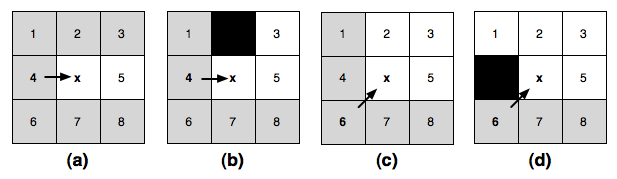
\includegraphics[scale=0.4, trim = 10mm 10mm 10mm 0mm]{diagrams/pruningrules.png}
       \end{center}
	\vspace{-3pt}
       \caption{A caption will eventually be here.}
       \label{fig:pruningrules}
\end{figure}


\subsection{Optimality}

We claim that the pruning rules we have developed thus far preserve both
completeness and optimality during search. 



